\chapter{Resultados}

Todos los resultados de este capítulo provienen de la ventana 1996-2025,
con la muestra de estimación descripta en la sección 4.5, y del
escenario base del análisis de sostenibilidad más reciente del FMI
(2026) para 2026-2035. La especificación principal mide la deuda federal
bruta, que parte de 80,3\% del PIB a fines de 2025, como en el FMI, y
usa el resultado primario sin rentas de la propiedad (sección 4.2). Los
intervalos son de 90\% y salen del \emph{bootstrap} descripto en la
sección 4.5. Los \emph{shocks} domésticos se identifican con
restricciones de impacto en la línea de Blanchard y Perotti (2002) para
el bloque fiscal y de actividad, con un bloque cambiario y de riesgo
(EMBI y TCRM) identificado en conjunto (sección 4.4).

\section{El SVARX estimado}

\textbf{Propiedades de las series.} El resultado primario se comporta
como una serie con raíz unitaria, el VIX como estacionaria, y en el
resto ADF y KPSS no coinciden (Apéndice, sección A.3), lo esperable en
series cortas con cambios de régimen (Perron, 1989). El procedimiento de
Bai y Perron (2003) encuentra quiebres en la deuda federal bruta en
2001T4, en 2006T2 y en 2018T1; Zivot y Andrews (1992) ubican uno en
2005T1, sin rechazar la raíz unitaria.

\textbf{Rezagos y diagnósticos.} Con dos rezagos (sección 4.5), el
sistema es estable: el autovalor máximo es 0,896, y su mediana entre las
réplicas del \emph{bootstrap}, 0,842. Los residuos no muestran
autocorrelación (Portmanteau, p = 0,056) ni heterocedasticidad
condicional al 5\% (ARCH-LM; Engle, 1982), pero rechazan la normalidad
multivariada (Jarque y Bera, 1987; p = 0,000), lo que justifica
remuestrear \emph{shocks} históricos (Apéndice, sección A.5).

\textbf{Reacción fiscal.} El coeficiente de la deuda rezagada en la
ecuación del resultado primario es el efecto de impacto de la deuda del
trimestre anterior sobre el resultado primario trimestral. Como el
resultado primario depende también de sus propios rezagos, el
multiplicador de largo plazo es mayor (Tabla 6.1; Apéndice, sección
A.7). Los dos son positivos, con intervalos que excluyen el cero, en los
dos perímetros.

\textbf{Tabla 6.1. Reacción fiscal según el perímetro de la deuda}

{\def\LTcaptype{none} % do not increment counter
\begin{longtable}[]{@{}
  >{\raggedright\arraybackslash}p{(\linewidth - 8\tabcolsep) * \real{0.2000}}
  >{\raggedright\arraybackslash}p{(\linewidth - 8\tabcolsep) * \real{0.2000}}
  >{\raggedright\arraybackslash}p{(\linewidth - 8\tabcolsep) * \real{0.2000}}
  >{\raggedright\arraybackslash}p{(\linewidth - 8\tabcolsep) * \real{0.2000}}
  >{\raggedright\arraybackslash}p{(\linewidth - 8\tabcolsep) * \real{0.2000}}@{}}
\toprule\noalign{}
\begin{minipage}[b]{\linewidth}\raggedright
Perímetro
\end{minipage} & \begin{minipage}[b]{\linewidth}\raggedright
Impacto
\end{minipage} & \begin{minipage}[b]{\linewidth}\raggedright
Intervalo de 90\%
\end{minipage} & \begin{minipage}[b]{\linewidth}\raggedright
Largo plazo
\end{minipage} & \begin{minipage}[b]{\linewidth}\raggedright
Intervalo de 90\%
\end{minipage} \\
\midrule\noalign{}
\endhead
\bottomrule\noalign{}
\endlastfoot
Deuda federal bruta (principal) & 0,0576 & {[}0,0220; 0,0822{]} & 0,199
& {[}0,112; 0,328{]} \\
Deuda consolidada con el BCRA (extensión) & 0,0595 & {[}0,0141;
0,0868{]} & 0,223 & {[}0,063; 0,375{]} \\
\end{longtable}
}

Fuente: elaboración propia.

El signo coincide con el que encuentran Celasun et al.~(2006) en su
panel de economías emergentes. Una reacción positiva es condición
suficiente para la solvencia en el sentido de Bohn (1998, 2005), pero no
dice si alcanza para estabilizar la deuda frente a los \emph{shocks} que
enfrenta.

\textbf{Retroalimentación de la deuda.} La deuda rezagada entra en las
cuatro ecuaciones del sistema (Favero y Giavazzi, 2007). Fuera de la
ecuación fiscal, ningún efecto se distingue del cero. Para el riesgo
país, medido por el diferencial del índice EMBI de J.P. Morgan para
Argentina (EMBI), la estimación puntual es de unos 15 puntos básicos por
punto de deuda, con un intervalo que va de -5 a 30: con la muestra
disponible no se puede afirmar que una deuda mayor eleve el EMBI. El
intervalo del crecimiento también incluye el cero, y con el tipo de
cambio real multilateral (TCRM) no hay relación.

\textbf{Respuesta a la tasa de la FED.} Un aumento de un desvío estándar
en la variación de la tasa de política monetaria de la Reserva Federal
(FED), de 0,494 puntos, no produce respuestas sistemáticas de las
variables domésticas (Figura 6.1). De las 84 respuestas estimadas
(cuatro variables en 21 horizontes), dos tienen un intervalo que excluye
el cero, ambas del TCRM, dos y tres trimestres después del \emph{shock},
y con signo de apreciación real. Con intervalos de 90\%, el azar
produciría más exclusiones aunque la FED no tuviera efecto, y el signo
contradice la teoría. El modelo no distingue los efectos indirectos de
la FED del ruido.

\begin{figure}
\centering
\pandocbounded{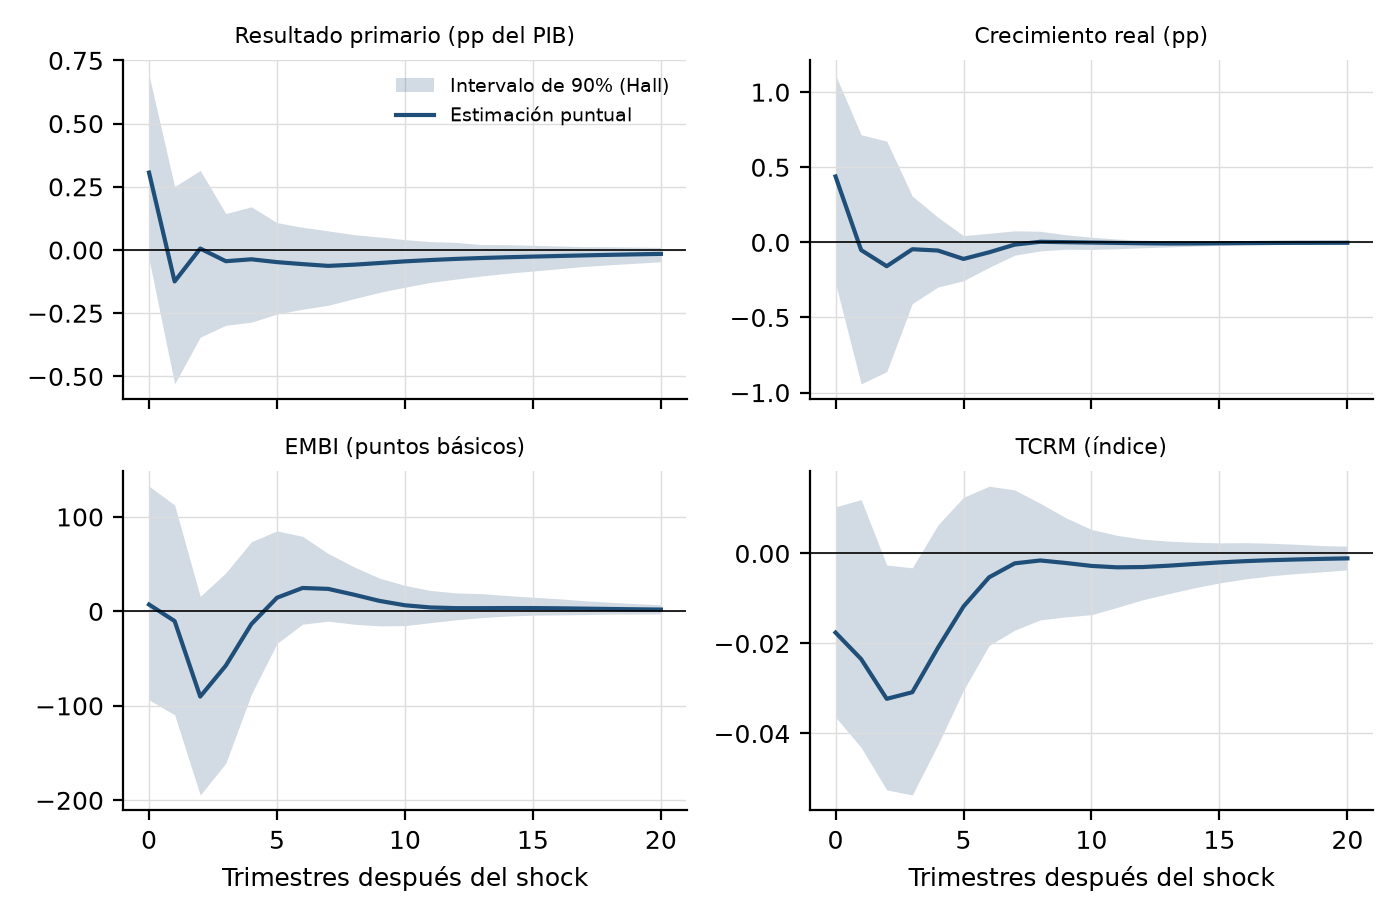
\includegraphics[keepaspectratio,alt={Respuestas al impulso ante una suba de la tasa de la FED. Aumento de un desvío estándar (0,494 puntos porcentuales) en la variación trimestral de la tasa; deuda federal bruta, dos rezagos, parámetros de mínimos cuadrados e intervalos de 90\% del bootstrap. Fuente: elaboración propia.}]{fig6_1_respuesta_fed.png}}
\caption[Respuestas al impulso ante una suba de la tasa de la FED]{Respuestas al impulso ante una suba de la tasa de la FED.
Aumento de un desvío estándar (0,494 puntos porcentuales) en la
variación trimestral de la tasa; deuda federal bruta, dos rezagos,
parámetros de mínimos cuadrados e intervalos de 90\% del
\emph{bootstrap}. Fuente: elaboración propia.}
\end{figure}

\section{El gráfico de abanico}

La Tabla 6.2 y la Figura 6.2 muestran la distribución de la deuda
simulada. La mediana baja de 80,3\% del PIB en 2025 a 53,1\% en 2031 y a
42,1\% en 2035, cerca de la senda determinista del escenario base
(53,9\% y 42,7\%). La caída la determina el escenario del FMI (2026,
cuadro 6), con superávit primario sostenido y una tasa de interés
efectiva menor que la inflación. La distribución es asimétrica hacia
arriba: en 2035 la deuda media es 45,3\%, por encima de la mediana, y el
percentil 95 supera el punto de partida.

\textbf{Tabla 6.2. Deuda federal bruta simulada (\% del PIB),
percentiles}

{\def\LTcaptype{none} % do not increment counter
\begin{longtable}[]{@{}llllll@{}}
\toprule\noalign{}
Año & p5 & p25 & Mediana & p75 & p95 \\
\midrule\noalign{}
\endhead
\bottomrule\noalign{}
\endlastfoot
2026 & 65,9 & 69,2 & 72,8 & 75,8 & 90,2 \\
2028 & 52,0 & 60,0 & 65,0 & 70,5 & 83,1 \\
2031 & 33,2 & 44,5 & 53,1 & 62,7 & 79,8 \\
2033 & 24,0 & 37,2 & 48,0 & 59,9 & 81,8 \\
2035 & 15,9 & 30,0 & 42,1 & 57,3 & 85,5 \\
\end{longtable}
}

Fuente: elaboración propia. Estimación central, 20.000 trayectorias.

\begin{figure}
\centering
\pandocbounded{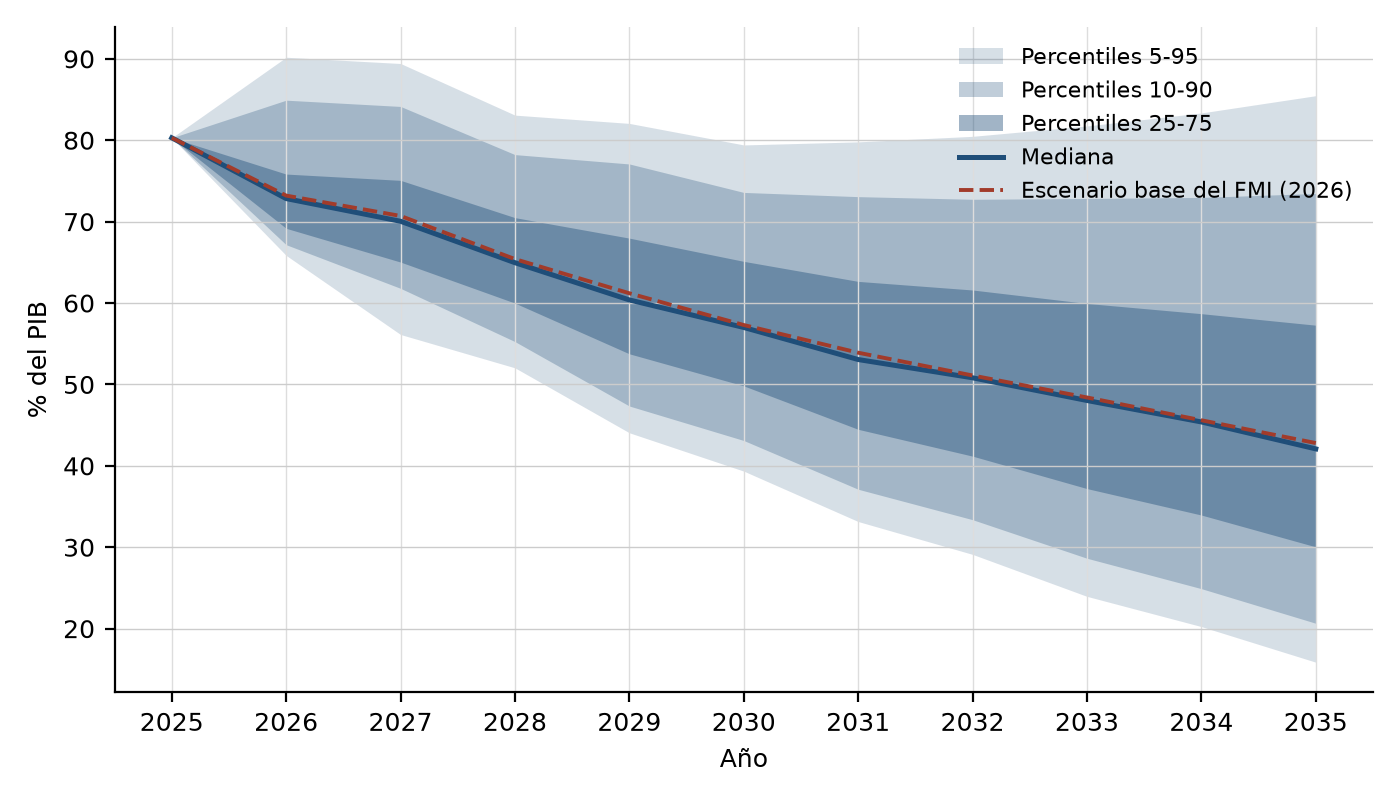
\includegraphics[keepaspectratio,alt={Gráfico de abanico de la deuda federal bruta simulada, 2025-2035 (\% del PIB). Escenario base del FMI (2026) con shocks estructurales del SVARX y variables externas simuladas; estimación central con parámetros de mínimos cuadrados y 20.000 trayectorias. La línea discontinua es la senda base del FMI. Fuente: elaboración propia.}]{fig6_2_abanico_deuda.png}}
\caption[Gráfico de abanico de la deuda federal bruta simulada, 2025-2035 (\% del PIB)]{Gráfico de abanico de la deuda federal bruta simulada,
2025-2035 (\% del PIB). Escenario base del FMI (2026) con \emph{shocks}
estructurales del SVARX y variables externas simuladas; estimación
central con parámetros de mínimos cuadrados y 20.000 trayectorias. La
línea discontinua es la senda base del FMI. Fuente: elaboración propia.}
\end{figure}

El ancho del abanico entre los percentiles 5 y 95 es de 46,6 puntos en
2031, con un intervalo de {[}36,8; 61,0{]}. El del FMI para la misma
deuda es 71,5 (FMI, 2026, cuadro 7). El Capítulo 7 analiza por qué un
abanico más angosto convive con una probabilidad de no estabilización
mayor.

\section{Contraste de H1a}

H1a sostiene que el superávit primario, por sí solo, no basta para
estabilizar la deuda, porque la condicionan también el crecimiento, el
TCRM y el riesgo país. La Tabla 6.3 descompone la varianza de la deuda
simulada en 2035 según el bloque de \emph{shocks}. El bloque externo
explica 44,9\% y el cambiario y de riesgo 32,3\%; el de actividad,
12,0\%, y el fiscal, 10,8\%. La diferencia entre los \emph{shocks} no
fiscales y el fiscal es de 78,3 puntos, con un intervalo de {[}57,3;
87,9{]} que excluye el cero. H1a queda respaldada.

\textbf{Tabla 6.3. Participación de cada bloque de \emph{shocks} en la
varianza de la deuda en 2035}

{\def\LTcaptype{none} % do not increment counter
\begin{longtable}[]{@{}lll@{}}
\toprule\noalign{}
Bloque de \emph{shocks} & Participación & Intervalo de 90\% \\
\midrule\noalign{}
\endhead
\bottomrule\noalign{}
\endlastfoot
Fiscal & 10,8\% & {[}6,1; 21,3{]} \\
Actividad & 12,0\% & {[}0,2; 21,2{]} \\
Cambiario y de riesgo (EMBI y TCRM) & 32,3\% & {[}16,8; 48,9{]} \\
Externo (FED y VIX) & 44,9\% & {[}14,6; 59,0{]} \\
No fiscal menos fiscal (diferencia) & 78,3 puntos & {[}57,3; 87,9{]} \\
\end{longtable}
}

Fuente: elaboración propia.

El resultado se sostiene en las 20 especificaciones (sección 6.6). El
menor límite inferior, 25,6 puntos, aparece cuando el \emph{shock}
fiscal absorbe toda la covarianza entre el resultado primario y el
crecimiento: en la variante de robustez con elasticidad cíclica de cero
o, de manera equivalente, con el ordenamiento de Cholesky que pone
primero al resultado primario.

\textbf{Suficiencia del superávit.} El análisis complementario,
descriptivo, desplaza en la misma magnitud el resultado primario de
todos los años del escenario base (Figura 6.3). El máximo anual de
1996-2025 es 3,29\% del PIB, en 2004, con la definición de la tesis (sin
rentas de la propiedad); con rentas de la propiedad es 3,58\%, el mismo
año. Con el resultado primario en ese nivel todos los años, la
probabilidad de no estabilización en 2031 es 26,1\%, y 24,5\% con el
máximo de la variante con rentas. Para llevarla al 1\% que estima el FMI
para Argentina hay que sumar 8,00 puntos al resultado primario del
escenario en todos los años: un superávit de 9,4\% del PIB en 2026 y de
10,3\% en 2031, más del triple del máximo observado.

La relación en 2035 no es monótona. La probabilidad baja hasta 0,71\%
con un desplazamiento de 6,50 puntos y vuelve a subir, a 2,91\% con
10,00 puntos. Con superávits tan altos la deuda queda cerca de cero, y
la métrica, que compara el resultado primario necesario con el previsto
año por año, se activa con \emph{shocks} pequeños.

\begin{figure}
\centering
\pandocbounded{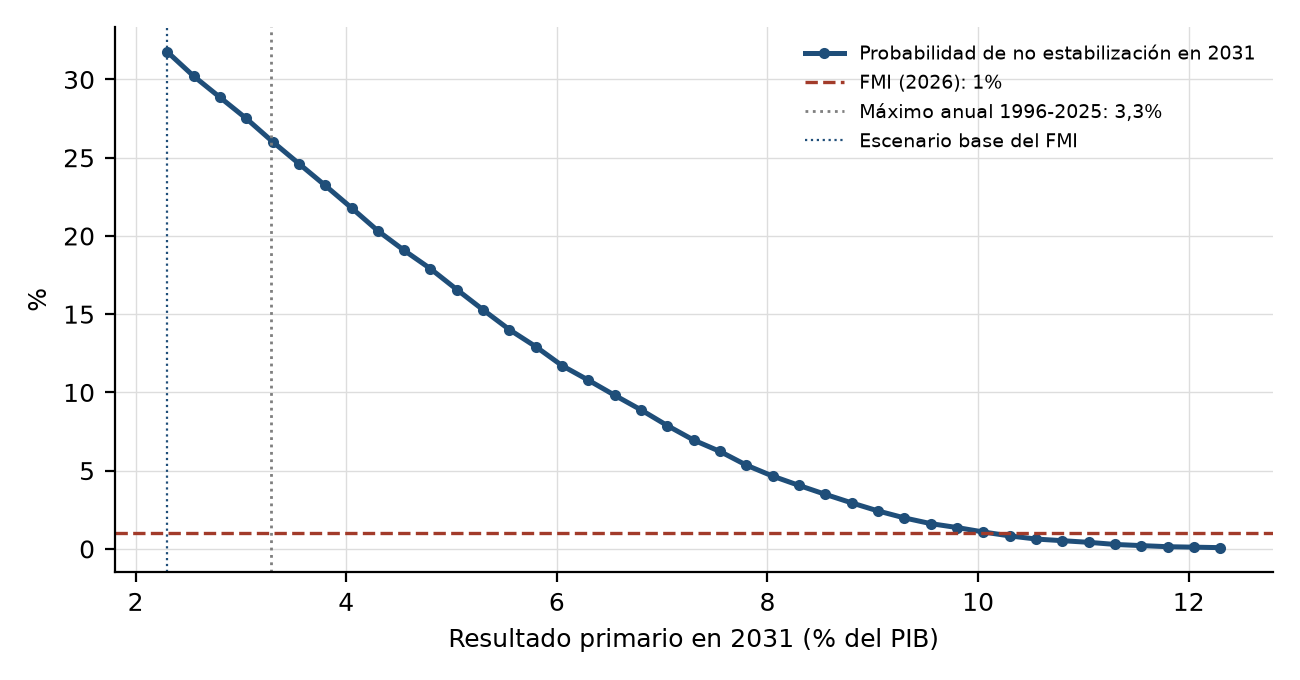
\includegraphics[keepaspectratio,alt={Suficiencia del superávit primario. Probabilidad de no estabilización en 2031 según el resultado primario de 2031, con el resultado primario de todos los años del escenario base del FMI (2026) desplazado en la misma magnitud; la línea vertical marca el máximo anual de 1996-2025. Estimación central. Fuente: elaboración propia.}]{fig6_5_suficiencia_superavit.png}}
\caption[Suficiencia del superávit primario]{Suficiencia del superávit primario. Probabilidad de no
estabilización en 2031 según el resultado primario de 2031, con el
resultado primario de todos los años del escenario base del FMI (2026)
desplazado en la misma magnitud; la línea vertical marca el máximo anual
de 1996-2025. Estimación central. Fuente: elaboración propia.}
\end{figure}

En la descomposición (Figura 6.4), los intervalos de los bloques externo
y cambiario y de riesgo se superponen y no permiten ordenarlos entre sí.

\begin{figure}
\centering
\pandocbounded{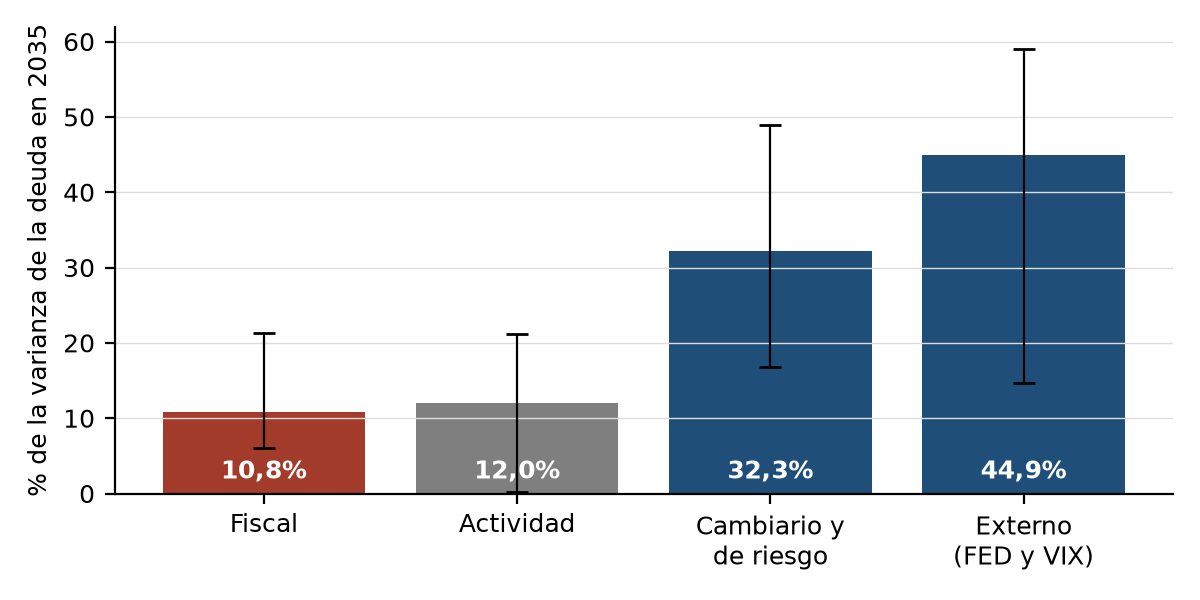
\includegraphics[keepaspectratio,alt={Varianza de la deuda en 2035 por bloque de shocks. Participación de los bloques fiscal, de actividad, cambiario y de riesgo, y externo en la varianza de la deuda federal bruta simulada en 2035; estimación central e intervalos de 90\%. Fuente: elaboración propia.}]{fig6_3_varianza_por_bloque.png}}
\caption[Varianza de la deuda en 2035 por bloque de \emph{shocks}. Participación de los bloques fiscal, de actividad, cambiario y de riesgo, y externo en la varianza de la deuda federal bruta simulada en 2035; estimación central e intervalos de 90\%. Fuente: elaboración propia]{Varianza de la deuda en 2035 por bloque de \emph{shocks}.
Participación de los bloques fiscal, de actividad, cambiario y de
riesgo, y externo en la varianza de la deuda federal bruta simulada en
2035; estimación central e intervalos de 90\%. Fuente: elaboración
propia.}
\end{figure}

\section{Contraste de H1b}

El FMI (2026) estima una probabilidad de no estabilización de 1\% en su
abanico de mediano plazo (cuadro 7) y menor que 3\% en su abanico de
diez años, que termina en 2035. Con la deuda federal bruta, el mismo
punto de partida, el mismo escenario y la misma métrica, cada horizonte
se contrasta contra la cifra del FMI correspondiente (Tabla 6.4).

\textbf{Tabla 6.4. Contraste de H1b}

{\def\LTcaptype{none} % do not increment counter
\begin{longtable}[]{@{}
  >{\raggedright\arraybackslash}p{(\linewidth - 8\tabcolsep) * \real{0.2000}}
  >{\raggedright\arraybackslash}p{(\linewidth - 8\tabcolsep) * \real{0.2000}}
  >{\raggedright\arraybackslash}p{(\linewidth - 8\tabcolsep) * \real{0.2000}}
  >{\raggedright\arraybackslash}p{(\linewidth - 8\tabcolsep) * \real{0.2000}}
  >{\raggedright\arraybackslash}p{(\linewidth - 8\tabcolsep) * \real{0.2000}}@{}}
\toprule\noalign{}
\begin{minipage}[b]{\linewidth}\raggedright
Horizonte
\end{minipage} & \begin{minipage}[b]{\linewidth}\raggedright
Probabilidad de no estabilización
\end{minipage} & \begin{minipage}[b]{\linewidth}\raggedright
Intervalo de 90\%
\end{minipage} & \begin{minipage}[b]{\linewidth}\raggedright
Cifra del FMI
\end{minipage} & \begin{minipage}[b]{\linewidth}\raggedright
Criterio
\end{minipage} \\
\midrule\noalign{}
\endhead
\bottomrule\noalign{}
\endlastfoot
2031 (mediano plazo) & 31,8\% & {[}25,2; 36,4{]} & 1\% & Se cumple \\
2035 (diez años) & 31,0\% & {[}26,8; 35,6{]} & menos de 3\% & Se
cumple \\
\end{longtable}
}

Fuente: elaboración propia. Error de Monte Carlo de la estimación
central: 0,33 puntos.

En los dos horizontes el intervalo queda entero muy por encima de la
cifra del FMI, y la conclusión se mantiene con la corrección de
Bonferroni (límites inferiores de 24,2\% y 26,6\%). Las medidas
alternativas llevan a lo mismo: con el resultado primario simulado en
lugar del previsto, la probabilidad en 2031 es 35,6\% {[}30,9; 41,1{]},
y la probabilidad de que la deuda de 2031 supere a la de 2029 es 25,8\%
{[}21,8; 31,2{]}. En las 20 especificaciones el límite inferior supera
las cifras del FMI; el menor, 19,1\%, corresponde a la deuda consolidada
con el BCRA. H1b queda respaldada en los dos horizontes.

\section{Contraste de H2}

\textbf{Tabla 6.5. Efecto de la FED sobre la deuda federal bruta}

{\def\LTcaptype{none} % do not increment counter
\begin{longtable}[]{@{}
  >{\raggedright\arraybackslash}p{(\linewidth - 6\tabcolsep) * \real{0.2500}}
  >{\raggedright\arraybackslash}p{(\linewidth - 6\tabcolsep) * \real{0.2500}}
  >{\raggedright\arraybackslash}p{(\linewidth - 6\tabcolsep) * \real{0.2500}}
  >{\raggedright\arraybackslash}p{(\linewidth - 6\tabcolsep) * \real{0.2500}}@{}}
\toprule\noalign{}
\begin{minipage}[b]{\linewidth}\raggedright
Escenario
\end{minipage} & \begin{minipage}[b]{\linewidth}\raggedright
Probabilidad en 2031 (pp)
\end{minipage} & \begin{minipage}[b]{\linewidth}\raggedright
Probabilidad en 2035 (pp)
\end{minipage} & \begin{minipage}[b]{\linewidth}\raggedright
Deuda media 2035 (pp del PIB)
\end{minipage} \\
\midrule\noalign{}
\endhead
\bottomrule\noalign{}
\endlastfoot
Nivel 0,494 pp más alto desde 2026T1 & +0,8 {[}0,1; 1,4{]} & +1,1
{[}0,2; 1,9{]} & +1,0 {[}0,0; 1,8{]} \\
Senda de 2022-2025 repetida en 2026-2029 & +5,0 {[}0,2; 9,2{]} & +9,7
{[}4,2; 16,0{]} & +9,0 {[}0,3; 16,2{]} \\
\end{longtable}
}

Fuente: elaboración propia. Diferencias respecto del escenario base;
entre corchetes, intervalos de 90\%.

Los dos escenarios elevan la probabilidad de no estabilización y la
deuda media en 2035 con intervalos que excluyen el cero, de modo que la
especificación principal cumple el criterio de la Tabla 4.4. En el
escenario de un desvío estándar el margen sobre la deuda es mínimo: el
límite inferior, positivo, se redondea a 0,0. El efecto en 2031 es
menor, como corresponde a un efecto que se acumula.

La evidencia se concentra en el efecto de la senda de 2022-2025 sobre la
probabilidad. Con la corrección de Bonferroni, ese efecto sigue
excluyendo el cero, con un intervalo de 95\% de {[}3,6; 16,8{]}. El del
escenario de un desvío estándar sobre la probabilidad ({[}-0,0; 2,0{]})
y los dos efectos sobre la deuda esperada ({[}-0,5; 2,0{]} y {[}-4,1;
17,4{]}) no lo excluyen. Entre las especificaciones de robustez, el
efecto de la senda sobre la probabilidad excluye el cero en 18 de 20;
las excepciones son los datos desde 2004 y la corrección de sesgo de
Kilian (1998). El efecto sobre la deuda lo excluye en 9 de 20.

Para saber por qué canal pasa el efecto, el escenario de 2022-2025 se
repitió anulando la respuesta de las variables domésticas a la FED, de
modo que solo actúa el mayor costo de la deuda en dólares. Ese costo
directo, que la identidad incorpora, explica 8,6 de los 9,0 puntos de
aumento de la deuda en 2035 (96\%). El resto corresponde a la respuesta
del EMBI, el TCRM y el crecimiento, que no se distinguen del azar
(sección 6.1). H2 queda respaldada en su efecto sobre la probabilidad de
no estabilización en el escenario de la senda de 2022-2025, que resiste
Bonferroni y casi todas las robusteces. El efecto sobre la deuda
esperada y el del escenario de un desvío estándar no son robustos, y el
mecanismo es el costo directo de la deuda en dólares; la transmisión por
los canales domésticos que propone la hipótesis no se verifica.

\section{Robustez}

La Tabla 6.6 resume las especificaciones alternativas más relevantes. La
tabla completa, con las 20 especificaciones del SVARX, las dos filas a
la manera del FMI y la cifra del FMI, está en el Apéndice, sección A.9.

\textbf{Tabla 6.6. Robustez (selección)}

{\def\LTcaptype{none} % do not increment counter
\begin{longtable}[]{@{}
  >{\raggedright\arraybackslash}p{(\linewidth - 12\tabcolsep) * \real{0.1429}}
  >{\raggedright\arraybackslash}p{(\linewidth - 12\tabcolsep) * \real{0.1429}}
  >{\raggedright\arraybackslash}p{(\linewidth - 12\tabcolsep) * \real{0.1429}}
  >{\raggedright\arraybackslash}p{(\linewidth - 12\tabcolsep) * \real{0.1429}}
  >{\raggedright\arraybackslash}p{(\linewidth - 12\tabcolsep) * \real{0.1429}}
  >{\raggedright\arraybackslash}p{(\linewidth - 12\tabcolsep) * \real{0.1429}}
  >{\raggedright\arraybackslash}p{(\linewidth - 12\tabcolsep) * \real{0.1429}}@{}}
\toprule\noalign{}
\begin{minipage}[b]{\linewidth}\raggedright
Especificación
\end{minipage} & \begin{minipage}[b]{\linewidth}\raggedright
No estabilización 2031
\end{minipage} & \begin{minipage}[b]{\linewidth}\raggedright
No estabilización 2035
\end{minipage} & \begin{minipage}[b]{\linewidth}\raggedright
Ancho en 2031
\end{minipage} & \begin{minipage}[b]{\linewidth}\raggedright
No fiscal menos fiscal
\end{minipage} & \begin{minipage}[b]{\linewidth}\raggedright
Senda de la FED: probabilidad 2035
\end{minipage} & \begin{minipage}[b]{\linewidth}\raggedright
Senda de la FED: deuda 2035
\end{minipage} \\
\midrule\noalign{}
\endhead
\bottomrule\noalign{}
\endlastfoot
Principal (deuda federal bruta) & 31,8\% {[}25,2; 36,4{]} & 31,0\%
{[}26,8; 35,6{]} & 46,6 & 78,3 {[}57,3; 87,9{]} & 9,7 {[}4,2; 16,0{]} &
9,0 {[}0,3; 16,2{]} \\
Deuda consolidada con el BCRA & 26,5\% {[}19,1; 30,5{]} & 24,1\%
{[}20,0; 30,0{]} & 37,3 & 70,2 {[}43,2; 80,9{]} & 10,1 {[}3,7; 17,2{]} &
6,3 {[}-0,2; 11,8{]} \\
Resultado primario con rentas de la propiedad & 32,0\% {[}25,7; 35,9{]}
& 31,3\% {[}27,4; 36,2{]} & 47,4 & 85,0 {[}70,3; 93,9{]} & 11,3 {[}5,3;
19,0{]} & 11,7 {[}2,1; 21,2{]} \\
Sin retroalimentación de la deuda & 30,4\% {[}24,8; 34,6{]} & 28,5\%
{[}23,6; 32,6{]} & 54,4 & 77,0 {[}54,7; 87,5{]} & 7,7 {[}4,7; 10,9{]} &
11,6 {[}4,1; 21,2{]} \\
Tres rezagos & 30,0\% {[}22,1; 34,5{]} & 29,5\% {[}24,3; 34,5{]} & 38,5
& 69,1 {[}40,3; 82,4{]} & 8,6 {[}4,3; 13,6{]} & 6,5 {[}1,1; 11,7{]} \\
Solo EMBI observado (datos desde 1999, sin empalme) & 32,4\% {[}26,6;
37,0{]} & 31,2\% {[}26,4; 35,6{]} & 47,6 & 75,5 {[}51,7; 86,3{]} & 9,6
{[}2,5; 15,7{]} & 9,6 {[}-0,6; 17,1{]} \\
Datos desde 2004 & 31,6\% {[}27,5; 39,5{]} & 31,8\% {[}24,0; 40,8{]} &
34,0 & 81,0 {[}62,2; 90,3{]} & 10,2 {[}-5,0; 16,7{]} & 6,7 {[}-29,8;
14,6{]} \\
Parámetros corregidos por sesgo (Kilian, 1998) & 30,1\% {[}24,3; 35,6{]}
& 31,4\% {[}25,3; 36,9{]} & 53,1 & 62,1 {[}29,4; 100,0{]} & 9,6 {[}-0,6;
18,6{]} & 9,4 {[}-9,1; 21,7{]} \\
\emph{Shocks} a la manera del FMI, deuda federal bruta & 24,1\% & 20,6\%
& 148,4 & no aplica & no aplica & no aplica \\
FMI (2026), deuda federal bruta & 1\% & menos de 3\% & 71,5 & no aplica
& no aplica & no aplica \\
\end{longtable}
}

Fuente: elaboración propia y FMI (2026, anexo II). Entre corchetes,
intervalos de 90\%. La fila a la manera del FMI no tiene intervalo
porque ese procedimiento no estima parámetros.

\textbf{Hipótesis.} H1b se cumple en todas las especificaciones. H1a
también: la diferencia entre los \emph{shocks} no fiscales y el fiscal
excluye el cero en las 20. El efecto de la senda de la FED sobre la
probabilidad solo incluye el cero con los datos desde 2004, la
especificación con menos observaciones, y con los parámetros corregidos
por sesgo; el efecto sobre la deuda esperada incluye el cero en 11 de
las 20. Las variantes de identificación, con dos ordenamientos de
Cholesky (resultado primario primero y resultado primario último) y
elasticidades cíclicas de 0 y 0,5, no modifican la probabilidad, porque
todas las especificaciones comparten el sorteo y los \emph{shocks}
estructurales reconstruyen los mismos residuos (sección 4.6); solo
cambia el reparto de la varianza entre bloques.

\textbf{Resultado primario con rentas de la propiedad.} Con la serie que
incluye las rentas de la propiedad, que contienen las utilidades del
BCRA en los años en que el Tesoro las registró como ingreso, la
probabilidad de no estabilización en 2031 es 32,0\% {[}25,7; 35,9{]},
contra 31,8\% con la definición de la tesis, y las tres hipótesis llevan
a las mismas conclusiones.

\textbf{Empalme del EMBI.} Con datos desde 1999, que usan solo el EMBI
observado, la probabilidad de no estabilización es 32,4\% {[}26,6;
37,0{]} en 2031, contra 31,8\% {[}25,2; 36,4{]} con la ventana completa,
y en 2035 es 31,2\%, contra 31,0\%. La diferencia entre los
\emph{shocks} no fiscales y el fiscal y el efecto de la senda de la FED
sobre la probabilidad siguen excluyendo el cero. Los resultados no
dependen de los empalmes de 1996-1998.

\textbf{Extensión consolidada.} Con la deuda consolidada con el BCRA,
que parte de 52,1\% del PIB, la senda base llega a 31,9\% en 2031 y a
21,8\% en 2035, y el abanico es más angosto que el federal. Las tres
hipótesis llevan a las mismas conclusiones que en la especificación
principal: la probabilidad de no estabilización supera con holgura las
cifras del FMI, la diferencia entre los \emph{shocks} no fiscales y el
fiscal excluye el cero y la senda de la FED eleva la probabilidad. Su
efecto sobre la deuda esperada, 6,3 puntos {[}-0,2; 11,8{]}, no excluye
el cero.

\textbf{Procedimiento del FMI.} Con \emph{shocks} generados a la manera
del FMI sobre la historia argentina de la ventana 1996-2025, la
probabilidad en 2031 es 24,1\%, unas tres cuartas partes de la del SVARX
y muy superior a la del FMI, con un abanico dos veces más ancho que el
del organismo (Capítulo 7).

\begin{figure}
\centering
\pandocbounded{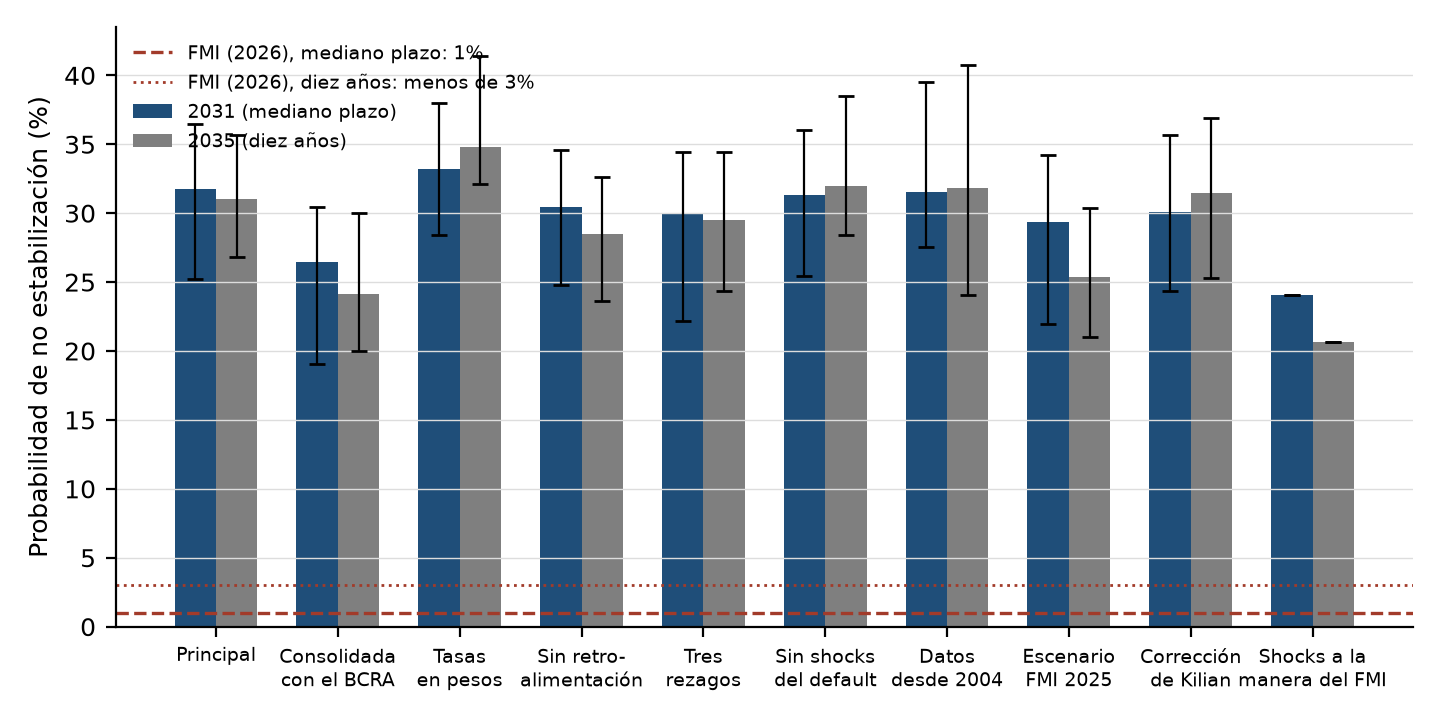
\includegraphics[keepaspectratio,alt={Probabilidad de no estabilización por especificación. Estimaciones centrales en 2031 y 2035 con intervalos de 90\%, y cifras del FMI (2026): 1\% a mediano plazo y menos de 3\% a diez años. La variante a la manera del FMI no tiene intervalo porque no estima parámetros. Fuente: elaboración propia.}]{fig6_4_probabilidad_no_estabilizacion.png}}
\caption[Probabilidad de no estabilización por especificación]{Probabilidad de no estabilización por especificación.
Estimaciones centrales en 2031 y 2035 con intervalos de 90\%, y cifras
del FMI (2026): 1\% a mediano plazo y menos de 3\% a diez años. La
variante a la manera del FMI no tiene intervalo porque no estima
parámetros. Fuente: elaboración propia.}
\end{figure}
